%Este trabalho está licenciado sob a Licença Atribuição-CompartilhaIgual 4.0 Internacional Creative Commons. Para visualizar uma cópia desta licença, visite http://creativecommons.org/licenses/by-sa/4.0/deed.pt_BR ou mande uma carta para Creative Commons, PO Box 1866, Mountain View, CA 94042, USA.

\chapter{Multiprocessamento (MP)}\label{cap_mp}
\thispagestyle{fancy}

Neste capítulo, vamos estudar aplicações da computação paralela em arquitetura de memória compartilhada. Para tanto, vamos discutir código C/C++ com a API \href{https://www.openmp.org/}{OpenMP}.

\section{Olá, Mundo!}\label{sec_ola_cap_mp}

A computação paralela com MP inicia-se por uma instância de processamento \emph{thread master}. Todas as instâncias de processamento disponíveis (\emph{threads}) leem e escrevem variáveis compartilhadas. A ramificação ({\it fork}) do processo entre os {\it threads} disponíveis é feita por instrução explícita no início de uma região paralela do código. Ao final da região paralela, todos os {\it threads} sincronizam-se ({\it join}) e o processo segue apenas com o {\it thread master}. Veja a Figura \ref{fig:mpwf}.

\begin{figure}[H]
  \centering
  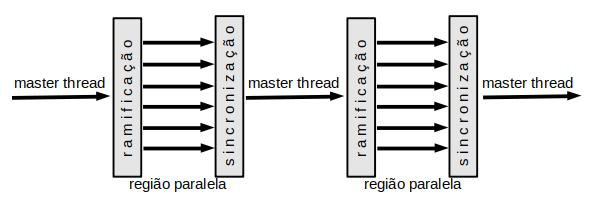
\includegraphics[width=0.7\textwidth]{./cap_mp/dados/fig_mpwf/mpwf}
  \caption{Fluxograma de um processo MP.}
  \label{fig:mpwf}
\end{figure}

Vamos escrever nosso primeiro programa MP. O Código \verb+ola.cc+ inicia uma região paralela e cada instância de processamento escreve ``Olá'' e identifica-se.

\lstinputlisting[title={Código: ola.cc}]{cap_mp/dados/cc_ola/ola.cc}

Na linha 4, o API OpenMP é incluído no código. A região paralela vale dentro do escopo iniciado pela instrução
\begin{verbatim}
# pragma omp parallel
\end{verbatim}
i.e., entre as linhas 12 e 17. Em paralelo, cada {\it thread} registra seu número de identificação na variável \verb+id+, veja a linha 14. Na linha 16, escrevem a saudação, identificando-se.

Para compilar este código, digite no terminal
\begin{verbatim}
$ g++ -fopenmp ola.cc
\end{verbatim}

Ao compilar, um executável \verb+a.out+ será criado. Para executá-lo, basta digitar no terminal:
\begin{verbatim}
$ a.out
\end{verbatim}

Ao executar, devemos ver a saída do terminal como algo parecido com\footnote{O código foi rodado em uma máquina Quadcore com 4 {\it threads}.}
\begin{verbatim}
Processo 0, olá!
Processo 3, olá!
Processo 1, olá!
Processo 2, olá!
\end{verbatim}

A saída irá depender do número de {\it threads} disponíveis na máquina e a ordem dos {\it threads} pode variar a cada execução. Execute o código várias vezes e analise as saídas!

\begin{obs}
  As variáveis declaradas dentro de uma região paralela são privadas de cada {\it threads}. As variáveis declaradas fora de uma região paralela são globais, sendo acessíveis por todos os {\it threads}.
\end{obs}

\subsection*{Exercícios resolvidos}

\begin{exeresol}
  O número de instâncias de processamento pode ser alterado pela variável do sistema \verb+OMP_NUM_THREADS+. Altere o número de {\it threads} para 2 e execute o Código ola.cc.
\end{exeresol}
\begin{resol}
  Para alterar o número de {\it threads}, pode-se digitar no terminal
\begin{verbatim}
$ export OMP_NUM_THREADS=2
\end{verbatim}
  Caso já tenha compilado o código, não é necessário recompilá-lo. Basta executá-lo com
\begin{verbatim}
$ ./a.out
\end{verbatim}
  A saída deve ser algo do tipo
\begin{verbatim}
Olá, processo 0
Olá, processo 1
\end{verbatim}
\end{resol}

\begin{exeresol}
  Escreva um código MP para ser executado com 2 {\it threads}. O {\it master thread} deve ler dois números em ponto flutuante. Então, em paralelo, um dos {\it threads} deve calcular a soma dos dois números e o outro thread deve calcular o produto.
\end{exeresol}
\begin{resol}
\lstinputlisting[title={Código: sp.cc}]{cap_mp/dados/cc_exeresol_sp/sp.cc}  
\end{resol}

\subsection*{Exercícios}

\begin{exer}
  Defina um número de {\it threads} maior do que o disponível em sua máquina. Então, rode o código \verb+ola.cc+ e analise a saída. O que você observa?
\end{exer}

\begin{exer}
  Modifique o código \verb+ola.cc+ de forma que cada {\it thread} escreva na tela ``Processo ID de NP, olá!'', onde ID é a identificação do {\it thread} e NP é o número total de {\it threads} disponíveis. O número total de {\it threads} pode ser obtido com a função OpenMP
\begin{verbatim}
omp_get_num_threads();
\end{verbatim}
\end{exer}

\begin{exer}
  Faça um código MP para ser executado com 2 threads. O {\it master thread} deve ler dois números $a$ e $b$ não nulos em ponto flutuante. Em paralelo, um dos {\it thread} de computar $a-b$ e o outro deve computar $a/b$. Por fim, o {\it master thread} deve escrever $(a-b) + (a/b)$.
\end{exer}

\begin{exer}\label{exer:cc_exer_Ax}
  Escreva um código MP para computar a multiplicação de uma matriz $n\times n$ com um vetor de $n$ elementos. Inicialize todos os elementos com números randômicos em ponto flutuante. Ainda, o código deve ser escrito para um número arbitrário $m>1$ de instâncias de processamento. Por fim, compare o desempenho do código MP com uma versão serial do código.
\end{exer}

\begin{exer}\label{exer:cc_exer_AB}
  Escreva um código MP para computar o produto de uma matriz $n\times m$ com uma matriz de $m\times n$ elementos, com $n \geq m$. Inicialize todos os elementos com números randômicos em ponto flutuante. Ainda, o código deve ser escrito para um número arbitrário $m>1$ de instâncias de processamento. Por fim, compare o desempenho do código MP com uma versão serial do código.
\end{exer}

\section{Construtores básicos}\label{cap_mp_sec_cb}

\subsection{Variáveis privadas e variáveis compartilhadas}

Vamos analisar o seguinte código.

\lstinputlisting[title={Código: vpc.cc}]{cap_mp/dados/cc_vpc/vpc.cc}

Qual seria a saída esperada? Ao rodarmos este código, veremos uma saída da forma
\begin{verbatim}
Processo 0/4
Processo 2/4
Processo 3/4
Processo 3/4
\end{verbatim}
Isto ocorre por uma situação de \emph{condição de corrida} (\emph{race condition}) entre os {\it threads}. As variáveis \verb+tid+ e \verb+nt+ foram declaradas antes da região paralela e, desta forma, são \emph{variáveis compartilhadas} (\emph{shared variables}) entre todos os {\it threads} na região paralela. Os locais na memória em que estas as variáveis estão alocadas é o mesmo para todos os {\it threads}.

A condição de corrida ocorre na linha 11. No caso da saída acima, as instâncias de processamento 1 e 3 entraram em uma condição de corrida no registro da variável \verb+tid+.

\begin{obs}
  Devemos estar sempre atentos a uma possível condição de corrida. Este é um erro comum no desenvolvimento de códigos em paralelo.
\end{obs}

Para evitarmos a condição de corrida, precisamos tornar a variável \verb+tid+ privada na região paralela. I.e., cada {\it thread} precisa ter uma variável \verb+tid+ privada. Podemos fazer isso alterando a linha 9 do código para
\begin{verbatim}
#pragma omp parallel private(tid)
\end{verbatim}
Com essa alteração, a saída terá o formato esperado, como por exemplo
\begin{verbatim}
Processo 0/4
Processo 3/4
Processo 2/4
Processo 1/4
\end{verbatim}
Faça a alteração e verifique!

\begin{obs}
  A diretiva \verb+#pragma omp parallel+ também aceita as instruções:
  \begin{itemize}
  \item \verb+default(private|shared|none)+: o padrão é \verb+shared+;
  \item \verb+shared(var1, var2, ..., varn)+: para especificar explicitamente as variáveis que devem ser compartilhadas. 
  \end{itemize}
\end{obs}

\subsection{Laço e Redução}

Vamos considerar o problema de computar
\begin{equation}
  s = \sum_{i=0}^{99999999} 1
\end{equation}
em paralelo com $np$ {\it threads}. Começamos analisando o seguinte código

\lstinputlisting[title={Código: soma0.cc}]{cap_mp/dados/cc_soma/soma0.cc}

Ao executarmos este código com $nt > 1$, vamos ter saídas erradas. Verifique! Qual o valor esperado?

O erro do código está na \emph{condição de corrida} ({\it race condition}) na linha 20. Esta é uma operação, ao ser iniciada por um {\it thread}, precisa ser terminada pelo {\it thread} antes que outro possa iniciá-la. Podemos fazer adicionando o construtor
\begin{verbatim}
#pragma omp critical
\end{verbatim}
imediatamente antes da linha de código \verb-s += i;-. O código fica como segue, verifique!

\lstinputlisting[title={Código: soma1.cc}]{cap_mp/dados/cc_soma/soma1.cc}

Esta abordagem evita a condição de corrida e fornece a resposta esperada. No entanto, ela acaba serializando o código, o qual é será muito mais lento que o código serial. Verifique!

\begin{obs}
  A utilização do construtor
\begin{verbatim}
#pragma omp critical
\end{verbatim}
  reduz a performance do código e só deve ser usada quando realmente necessária.
\end{obs}

Uma alternativa é alocar as somas parciais de cada {\it thread} em uma variável privada e, ao final, somar as partes computadas. Isto pode ser feito com o seguinte código. Verifique!

\lstinputlisting[title={Código: soma2.cc}]{cap_mp/dados/cc_soma/soma2.cc}

Este último código pode ser simplificado usando o construtor
\begin{verbatim}
#pragma omp for
\end{verbatim}
Com este construtor, o laço do somatório pode ser automaticamente distribuindo entre os {\it threads}. Verifique o seguinte código!

\lstinputlisting[title={Código: somafor.cc}]{cap_mp/dados/cc_soma/somafor.cc}

Mais simples e otimizado, é automatizar a operação de redução (no caso, a soma das somas parciais) adicionado
\begin{verbatim}
reduction(+: s)
\end{verbatim}
ao construtor que inicializa a região paralela. Verifique o seguinte código!

\lstinputlisting[title={Código: soma.cc}]{cap_mp/dados/cc_soma/soma.cc}

\begin{obs}
  A instrução de redução pode ser usada com qualquer operação binária aritmética (\verb=+=, \verb=-=, \verb=/=, \verb=*=), lógica (\verb=&=, \verb=|=) ou procedimentos intrínsecos (\verb=max=, \verb=min=).
\end{obs}

\subsection{Sincronização}

A sincronização dos {\it threads} deve ser evitada sempre que possível, devido a perda de performance em códigos paralelos. Atenção, ela ocorre implicitamente no término da região paralela!

\subsubsection{Barreira}

No seguinte código, o {\it thread} 1 é atrasado em 1 segundo, de forma que ele é o último a imprimir. Verifique!

\lstinputlisting[title={Código: sinc0.cc}]{cap_mp/dados/cc_sinc/sinc0.cc}

Agora, podemos forçar a sincronização dos {\it threads} usando o construtor
\begin{verbatim}
#pragma omp barrier
\end{verbatim}
em uma determinada linha do código. Por exemplo, podemos fazer todos os {\it threads} esperarem pelo {\it thread} 1 no código acima. Veja a seguir o código modificado. Teste!

\lstinputlisting[title={Código: sinc1.cc}]{cap_mp/dados/cc_sinc/sinc1.cc}

\subsubsection{Seção}

O construtor \verb+sections+ pode ser usado para determinar seções do código que deve ser executada de forma serial apenas uma vez por um único {\it thread}. Verifique o seguinte código.

\lstinputlisting[title={Código: secao.cc}]{cap_mp/dados/cc_secao/secao0.cc}

No código acima, o primeiro {\it thread} que alcançar a linha 19 é o único a executar a seção 1 e, o primeiro que alcançar a linha 25 é o único a executar a seção 2.

Observe que ocorre a sincronização implícita de todos os {\it threads} ao final do escopo \verb+sections+. Isso pode ser evitado usando a cláusula \verb+nowait+, i.e. alterando a linha 16 para
\begin{verbatim}
# pragma omp sections nowait
\end{verbatim}
Teste!

\begin{obs}
  A clausula \verb+nowait+ também pode ser usada com o construtor \verb+for+, i.e.
\begin{verbatim}
#pragma omp for nowait
\end{verbatim}
\end{obs}

Para uma região contendo apenas uma seção, pode-se usar o construtor
\begin{verbatim}
#pragma omp single
\end{verbatim}
Isto é equivalente a escrever
\begin{verbatim}
#pragma omp sections
  #pragma omp section
\end{verbatim}

\subsection*{Exercícios Resolvidos}

\begin{exeresol}\label{exeresol:produto_escalar}
  Escreva um código MP para computar o produto escalar entre dois vetores de $n$ pontos flutuantes randômicos.
\end{exeresol}
\begin{resol}
  Aqui, vamos usar o suporte a vetores e números randômicos do pacote de computação cientifica \href{https://www.gnu.org/software/gsl/}{GSL}. A solução é dada no código a seguir.

  \lstinputlisting[title={Código: prodesc.cc}]{cap_mp/dados/cc_prodesc/prodesc.cc}

  Para compilar o código acima, digite
\begin{verbatim}
$ g++ -fopenmp prodesc.cc -lgsl -lgslcblas
\end{verbatim}
\end{resol}

\begin{exeresol}\label{exeresol:cc_AxSecoes}
  Faça um código MP para computar a multiplicação de uma matriz $A$ $n\times n$ por um vetor de $n$ elementos (pontos flutuantes randômicos). Utilize o construtor \verb+omp sections+ para distribuir a computação entre somente dois {\it threads}.
\end{exeresol}
\begin{resol}
  Vamos usar o suporte a matrizes, vetores, BLAS e números randômicos do pacote de computação científica \href{https://www.gnu.org/software/gsl/}{GSL}. A solução é dada no código a seguir.

  \lstinputlisting[title={Código: AxSecoes.cc}]{cap_mp/dados/cc_AxSecoes/AxSecoes.cc}
\end{resol}

\subsection*{Exercícios}

\begin{exer}
  Considere o seguinte código
  \begin{lstlisting}
    int tid = 10;
    #pragma omp parallel private(tid)
    {
      tid = omp_get_thread_num();
    }
    printf("%d\n", tid);
  \end{lstlisting}
  Qual o valor impresso?
\end{exer}

\begin{exer}\label{exer:cc_trap}
  Escreva um código MP para computar uma aproximação para
  \begin{equation}
    I = \int_{-1}^{1} e^{-x^2}\,dx
  \end{equation}
  usando a \href{https://phkonzen.github.io/notas/MatematicaNumerica/cap_integr_sec_int_comp.html}{regra composta do trapézio} com $n$ subintervalos uniformes.
\end{exer}

\begin{exer}\label{exer:cc_simp}
  Escreva um código MP para computar uma aproximação para
  \begin{equation}
    I = \int_{-1}^{1} e^{-x^2}\,dx
  \end{equation}
  usando a \href{https://phkonzen.github.io/notas/MatematicaNumerica/cap_integr_sec_int_comp.html}{regra composta de Simpson} com $n$ subintervalos uniformes. Dica: evite sincronizações desnecessárias!
\end{exer}

\begin{exer}\label{exer:cc_Ax}
  Escreva um código MP para computar a multiplicação de uma matriz $A$ $n\times n$ por um vetor $x$ de $n$ elementos (pontos flutuantes randômicos). Faça o código de forma a suportar uma arquitetura com $n_p \geq 1$ {\it threads}. 
\end{exer}

\begin{exer}
  Escreva um código MP para computar o produto de duas matrizes $n\times n$ de pontos flutuantes randômicos. Utilize o construtor \verb+omp sections+ para distribuir a computação entre somente dois {\it threads}. 
\end{exer}

\begin{exer}
  Escreva um código MP para computar o produto de duas matrizes $n\times n$ de pontos flutuantes randômicos. Faça o código de forma a suportar uma arquitetura com $n_p \geq 1$ {\it threads}.
\end{exer}

\section{Resolução de Sistema Linear Triangular}\label{cap_mp_sec_sistria}

Nesta seção, vamos discutir sobre a uma implementação em paralelo do método da substituição para a resolução de sistemas triangulares. Primeiramente, vamos considerar $A$ uma matriz triangular inferior quadrada de dimensões $n\times n$, i.e. $A=[a_{i,j}]_{i,j=0}^{n-1}$ com $a_{i,j}=0$ para $i<j$. Ainda, vamos considerar que $A$ é invertível.

Neste caso, um sistema linear $Ax = b$ pode ser escrito na seguinte forma algébrica
\begin{gather}
  a_{1,1}x_1 = b_1\\
             \vdots \\
  a_{i,1}x_1 + a_{i,2}x_2 + \cdots + a_{i,i-1}x_{i-1} + a_{i,i}x_{i} = b_i \\
             \vdots\\
  a_{n,1}x_1 + a_{n,2}x_2 + \cdots + a_{i,i}x_i + \cdots + a_{n,n}x_{n} = b_n               
\end{gather}

O algoritmo serial do método da substituição (para frente) resolve o sistema começando pelo cálculo de $x_1$ na primeira equação, então o cálculo de $x_2$ pela segunda equação e assim por diante até o cálculo de $x_n$ pela última equação. Segue o pseudocódigo serial.
\begin{enumerate}
\item Para $i = 0, \dotsc, n-1$:
  \begin{enumerate}
  \item Para $j = 0, \dotsc, i-1$:
    \begin{enumerate}
    \item $b_i = b_i - A_{i,j}x_j$
    \end{enumerate}
  \item $\displaystyle x_i = \frac{b_i}{A_{i,i}}$
  \end{enumerate}
\end{enumerate}
Implemente!

Para o algoritmo paralelo, vamos considerar uma arquitetura MP com $n_p \geq 1$ instâncias de processamento. Para cada instância de processamento $1 \leq p_{id} < n_p-1$ vamos alocar as seguintes colunas da matriz $A$
\begin{gather}
  t_{ini} = p_{id}\left\lfloor\frac{n}{n_p}\right\rfloor\\
  t_{fim} = (p_{id}+1)\left\lfloor\frac{n}{n_p}\right\rfloor-1 
\end{gather}
e, para $p_{id}=n_{p}-1$ vamos alocar as últimas colunas, i.e.
\begin{gather}
  t_{ini} = p_{id}\left\lfloor\frac{n}{n_p}\right\rfloor\\
  t_{fim} = n-1
\end{gather}
Segue o pseudocódigo em paralelo.
\begin{enumerate}
\item Para $i = 0,\dotsc,n-1$
  \begin{enumerate}
  \item $s = 0$
  \item Região paralela
    \begin{enumerate}
    \item Para $j\in\{t_{ini},\dotsc,t_{fim}\}\land\{0,\dotsc,i-1\}$
      \begin{enumerate}
      \item $s = s + a_{i,j}x_{j}$
      \end{enumerate}
    \end{enumerate}
  \item $\displaystyle x_i = \frac{b_i - s}{a_{i,i}}$
  \end{enumerate}
\end{enumerate}

O código MP C/C++ que apresentaremos a seguir, faz uso do construtor \verb+threadprivate+
\begin{verbatim}
#pragma omp threadprivate(list)
\end{verbatim}
Este construtor permite que a lista de variáveis (estáticas) \verb+list+ seja privada para cada {\it thread} e seja compartilhada entre as regiões paralelas. Por exemplo:
\begin{verbatim}
x = 0
#pragma omp parallel private(x)
  x = 1
#pragma omp parallel private(x)
  x vale 0
\end{verbatim}
Agora, com o construtor \verb+threadprivate+:
\begin{verbatim}
static x = 0
#pragma omp threadprivate(x)
#pragma omp parallel
  x = 1
#pragma omp parallel private(x)
  x vale 1
\end{verbatim}

Ainda, apenas para efeito de exemplo, vamos considerar que $a_{i,j} = (-1)^{i+j}(i+j)/(ij+1)$ para $i<j$, $a_{i,i} = 2[(i-n/2)^2+1]/n$ e $b_i = (-1)^i/(i+1)$ para $i=0,\dotsc,n-1$.

Segue o código paralelo para a resolução direta do sistema triangular inferior. Verifique!

\lstinputlisting[title={Código: sistria1dcol.cc}]{cap_mp/dados/cc_sistria/sistria1dcol.cc}

\subsection*{Exercícios resolvidos}

\begin{exeresol}\label{exeresol:mp_sistria_1drow}
  Seja $Ax = b$ um sistema triangular inferior de dimensões $n\times n$. O seguinte pseudocódigo paralelo é uma alternativa ao apresentado acima. Por que este pseudocódigo é mais lento que o anterior?
  \begin{enumerate}
  \item Região paralela
    \begin{enumerate}
    \item Para $j = 0,\dotsc,n-1$
      \begin{enumerate}
      \item Se $j\in\{t_{ini},\dotsc,t_{fim}\}$
        \begin{enumerate}
        \item $\displaystyle x_j = \frac{b_j}{a_{j,j}}$
        \end{enumerate}
      \item Para $i\in\{t_{ini},\dotsc,t_{fim}\}\land\{j+1,\dotsc,n-1\}$
        \begin{enumerate}
        \item $b_i = b_i - a_{i,j}x_j$
        \end{enumerate}
      \end{enumerate}
    \end{enumerate}
  \end{enumerate}
\end{exeresol}
\begin{resol}
  Este código tem um número de operações semelhante ao anterior, seu desempenho é afetado pelo chamado compartilhamento falso ({\it false sharing}). Este é um fenômeno relacionado ao uso ineficiente da memória {\it cache} de cada {\it thread}. O último laço deste pseudocódigo faz sucessivas atualizações do vetor $b$, o que causa sucessivos recarregamentos de partes do vetor $b$ da memória RAM para a memória {\it cache} de cada um dos {\it threads}. Verifique!
\end{resol}

\begin{exeresol}
  Seja $A$ uma matriz triangular inferior e invertível de dimensões $n\times n$. Escreva um pseudocódigo MP para calcular a matriz inversa $A^{-1}$ usando o método de substituição direta.
\end{exeresol}
\begin{resol}
  Vamos denotar $A=[a_{i,j}]_{i,j=1}^{n-1}$ e $A^{-1} = [x_{i,j}]_{i,j=1}^{n-1}$. Note que $x's$ são as incógnitas. Por definição, $AA^{-1}=I$, logo
  \begin{gather}
    a_{1,1}x_{1,k} = \delta_{1,k}\\
    \cdots\\
    a_{i,1}x_{1,k}+\cdots+a_{i,i-1}x_{i-1,k}+a_{i,i}x_{i,k}=\delta_{i,k}\\
    \cdots\\
    a_{n-1,1}x_{1,k}+\cdots+a_{n-1,n-1}x_{n-1,k}=\delta_{n-1,k}
  \end{gather}
  onde, $k=0,\dotsc,n-1$ e $\delta_{i,j}$ denota o Delta de Kronecker. Ou seja, o cálculo de $A^{-1}$ pode ser feito pela resolução de $n$ sistemas triangulares inferiores tendo $A$ como matriz de seus coeficientes.

  Para construirmos um pseudocódigo MP, podemos distribuir os sistemas lineares a entre os {\it threads} disponíveis. Então, cada {\it thread} resolve em serial seus sistemas. Segue o pseudocódigo, sendo $x_k=(x_{1,k},\dotsc,x_{n-1,k})$ e $b_k = (\delta_{1,k},\dotsc,\delta_{n-1,k})$.
  \begin{enumerate}
  \item Região paralela
    \begin{enumerate}
    \item Para $k\in\{t_{ini},\dotsc,t_{fim}\}$
      \begin{enumerate}
      \item resolve $Ax_k=b_k$
      \end{enumerate}
    \end{enumerate}
  \end{enumerate}
\end{resol}

\subsection*{Exercícios}

\begin{exer}
  Implemente um código MP do pseudocódigo discutido no ER \ref{exeresol:mp_sistria_1drow}. Compare o tempo computacional com o do código \verb+sistria1dcol.cc+.
\end{exer}

\begin{exer}
  Implemente um código MP para computar a inversa de uma matriz triangular inferior de dimensões $n\times n$.
\end{exer}

\begin{exer}
  Implemente um código MP para computar a solução de um sistema linear triangular superior de dimensões $n\times n$.
\end{exer}

\begin{exer}
  Implemente um código MP para computar a inversa de uma matriz triangular superior de dimensões $n\times n$.
\end{exer}

\section{Decomposição LU}\label{cap_mp_sec_lu}

Nesta seção, vamos discutir sobre a paralelização da decomposição LU para matrizes. A decomposição $LU$ de uma matriz $A$ com dimensões $n\times n$ é
\begin{equation}
  A = LU
\end{equation}
onde $L$ é uma matriz triangular inferior e $U$ é uma matriz triangular superior, ambas com dimensões $n\times n$.

Para fixar as ideais, vamos denotar $A = [a_{i,j}]_{i,j=0}^{n-1}$, $L = [l_{i,j}]_{i,j=0}^{n-1}$ sendo $l_{i,i}=1$ e $l_{i,j}=0$ para $i>j$, e $U = [u_{i,j}]_{i,j=0}^n$ sendo $u_{i,j}=0$ para $i<j$. O pseudoalgoritmo serial para computar a decomposição $LU$ é
\begin{enumerate}
\item U = A, L = I
\item Para $k = 0,\dotsc, n-2$
  \begin{enumerate}
  \item Para $i = k+1,\dotsc,n-1$
    \begin{enumerate}
    \item $l_{i,k} = u_{i,k}/u_{k,k}$
    \item Para $j = k,\dotsc, n-1$
      \begin{enumerate}
      \item $u_{i,j} = u_{i,j} - l_{i,k}u_{k,j}$
      \end{enumerate}
    \end{enumerate}
  \end{enumerate}
\end{enumerate}

A forma mais fácil de paralelizar este algoritmo em uma arquitetura MP é paralelizando um de seus laços (itens 2., 2.(a) ou 2.(a)ii.). O laço do item 2. não é paralelizável, pois a iteração seguinte depende do resultado da iteração imediatamente anterior. Agora, os dois laços seguintes são paralelizáveis. Desta forma, o mais eficiente é paralelizarmos o segundo laço 2.(a).

O seguinte código é uma versão paralela da decomposição LU. A matriz $A$ é inicializada como uma matriz simétrica de elementos randômicos (linhas 19-41), sendo que a decomposição é computada nas linhas 43-61.

\lstinputlisting[title={Código: parallelLU.cc}]{cap_mp/dados/cc_lu/parallelLU.cc}

\subsection*{Exercícios Resolvidos}

\begin{exeresol}\label{exeresol:AxbLU}
  Faça um código MP para computar a solução de um sistema linear $Ax=b$ usando a decomposição LU. Assuma $A$ uma matriz simétrica $n\times n$ de elementos randômicos, assim como os elementos do vetor $b$.
\end{exeresol}
\begin{resol}
  A decomposição LU da matriz $A$ nos fornece as matrizes $L$ (matriz triangular inferior) e $U$ (matriz triangular superior), com
  \begin{equation}
    A = LU
  \end{equation}
  Logo, temos
  \begin{gather}
    Ax = b\\
    \Rightarrow (LU)x = b\\
    \Rightarrow L(Ux)=b
  \end{gather}
  Denotando $Ux = y$, temos que $y$ é solução do sistema triangular inferior
  \begin{equation}
    Ly = b
  \end{equation}
  e, por conseguinte, $x$ é solução do sistema triangular superior
  \begin{equation}
    Ux = y.
  \end{equation}

  Em síntese, o sistema $Ax=b$ pode ser resolvido com o seguinte pseudocódigo:
  \begin{enumerate}
  \item Computar a decomposição LU, A=LU.
  \item Resolver $Ly = b$.
  \item Resolver $Ux = b$.
  \end{enumerate}
  Cada passo acima pode ser paralelizado. O código MP fica de exercício, veja E \ref{exer:AxbLU}.  
\end{resol}

\begin{exeresol}\label{exeresol:parallelLU2}
  Considere a decomposição LU de uma matriz $A$ $n\times n$. Em muitas aplicações, não há necessidade de guardar a matriz $A$ em memória após a decomposição. Além disso, fixando-se que a diagonal da matriz $L$ tem todos os elementos iguais a 1, podemos alocar seus elementos não nulos na parte triangular inferior (abaixo da diagonal) da própria matriz $A$. E, a matriz $U$ pode ser alocada na parte triangular superior da matriz $A$. Faça um código MP para computar a decomposição LU de uma matriz $A$, alocando o resultado na própria matriz $A$.
\end{exeresol}
\begin{resol}
  O seguinte código faz a implementação pedida. Neste código, é necessário alocar apenas a matriz $A$, sem necessidade de locar as matrizes $L$ e $U$. Da linha 17 à 39, apenas é gerada a matriz randômica $A$. A decomposição é computada da linha 41 a 54.
  
  \lstinputlisting[title={Código: parallelLU2.cc}]{cap_mp/dados/cc_lu/parallelLU2.cc}

  Este algoritmo demanda substancialmente menos memória computacional que o código \verb+parallelLU.cc+ visto acima. Por outro lado, ele é substancialmente mais lento, podendo demandar até o dobro de tempo. Verifique!

  O aumento no tempo computacional se deve ao mau uso da memória {\it cache} dos processadores. A leitura de um elemento da matriz, aloca no {\it cache} uma sequência de elementos próximos na mesma linha. Ao escrever em um destes elementos, a alocação do {\it cache} é desperdiçada, forçando o {\it cache} a ser atualizado. Note que o código \verb+parallelLU.cc+ requer menos atualizações do {\it cache} que o código \verb+parallelLU2.cc+.
\end{resol}

\subsection*{Exercícios}

\begin{exer}\label{exer:AxbLU}
  Implemente o código MP discutido no ER \ref{exeresol:AxbLU}.
\end{exer}

\begin{exer}
  Implemente um código MP para computar a inversa de uma matriz simétrica de elementos randômicos usando decomposição LU.
\end{exer}

\begin{exer}
  Considere o pseudoalgoritmo serial da composição LU apresentado acima. Por que é melhor paralelizar o laço 2.(a) do que o laço o 2.(a)ii.?
\end{exer}

\begin{exer}
  Use o código MP discutido no ER \ref{exeresol:parallelLU2} para resolver um sistema $Ax=b$ de $n$ equações e $n$ incógnitas. Assuma que a matriz $A$ seja simétrica.
\end{exer}

\begin{exer}
  Um algoritmo paralelo mais eficiente para computar a decomposição LU pode ser obtido usando-se a decomposição LU por blocos. Veja o vídeo \href{https://youtu.be/E8aBJsC0bY8}{https://youtu.be/E8aBJsC0bY8} e implemente um código MP para computar a decomposição LU por blocos.
\end{exer}

\section{Métodos iterativos para Sistemas Lineares}\label{cap_mp_sec_mitsislin}

Nesta seção, vamos discutir sobre a paralelização MP de alguns métodos iterativos para sistemas lineares
\begin{equation}
  Ax = b
\end{equation}
com $A = [a_{i,j}]_{i,j=0}^{n-1}$, $x = (x_i)_{i=0}^{n-1}$ e $b=(b_i)_{i=0}^{n-1}$.

\subsection{Método de Jacobi}\label{subsec:mp_mitsislin_Jacobi}

Nós podemos escrever a $i$-ésima equação do sistema $Ax = b$ como
\begin{equation}
  \sum_{j=1}^n a_{i,j}x_j = b_i.
\end{equation}
Isolando $x_{i}$, obtemos
\begin{equation}\label{eq:mp_iterJacobi}
  x_i = -\frac{1}{a_{i,i}}\left[\sum_{j\neq i}a_{i,j}x_j - b_i\right].
\end{equation}

Nesta última equação, temos que $x_i$ pode ser diretamente calculado se todos os elementos $x_j$, $j\neq i$, forem conhecidos. Isso motiva o chamado método de Jacobi que é dado pela seguinte iteração
\begin{gather}
  x_i(0) = \text{aprox. inicial},\\
  x_i(t+1) = -\frac{1}{a_{i,i}}\left[\sum_{j\neq i}a_{i,j}x_j(t) - b_i\right],\label{eq:mp_jacobi_xi}
\end{gather}
para cada $i=0,1,\dotsc,n-1$ e $t=0,1,2,\ldots$. O número máximo de iterações $t_{\text{max}}$ e o critério de parada podem ser escolhidos de forma adequada.

O pseudocódigo serial para o método de Jacobi pode ser escrito como segue
\begin{enumerate}
\item Alocar a aproximação inicial $x^0$.
\item Para $t=0,1,2,\cdots,t_{\text{max}}$:
  \begin{enumerate}
  \item Para $i=0,1,2,\cdots,n$:
    \begin{enumerate}
    \item $\displaystyle x_i = -\frac{1}{a_{i,i}}\left[\sum_{j\neq i}a_{i,j}x^0_j - b_i\right]$.
    \end{enumerate}
  \item Verificar o critério de parada.
  \item $x0 = x$.
  \end{enumerate}
\end{enumerate}

A paralelização MP no método de Jacobi pode ser feita de forma direta e eficaz pela distribuição do laço 2.(a) do pseudocódigo acima. O seguinte código é uma implementação MP do método de Jacobi. Os vetores $b$ e $x0$ são inicializados com elementos randômicos $(0, 1)$. A matriz $A$ é inicializada como uma matriz estritamente diagonal dominante\footnote{O método de Jacobi é convergente para matriz estritamente diagonal dominante.} com elementos randômicos $(-1, 1)$. O critério de parada é
\begin{equation}
  \|x-x^0\|_2 < \text{tol},
\end{equation}
onde $\text{tol}$ é a tolerância.

\lstinputlisting[title={Código: pJacobi.cc}]{cap_mp/dados/cc_Jacobi/pJacobi.cc}

\subsection{Método {\it tipo} Gauss-Seidel}\label{subsec:mp_mitsislin_GS}

No algoritmo serial, observamos que ao calcularmos $x_i$ pela iteração de Jacobi\eqref{eq:mp_iterJacobi}, as incógnitas $x_j$, $j<i$, já foram atualizadas. Isto motivo o método de Gauss-Seidel, cujo algoritmo é descrito no seguinte pseudocódigo:
\begin{enumerate}
\item Alocar a aproximação inicial $x^0$.
\item Para $t=0,1,2,\cdots,t_{\text{max}}$:
  \begin{enumerate}
  \item Para $i=0,1,2,\cdots,n$:
    \begin{enumerate}
    \item $\displaystyle x_i = -\frac{1}{a_{i,i}}\left[\sum_{j<i}a_{i,j}x_j + \sum_{j>i}a_{i,j}x^0_j - b_i\right]$.
    \end{enumerate}
  \item Verificar o critério de parada.
  \item $x0 = x$.
  \end{enumerate}
\end{enumerate}

Embora este método seja normalmente muito mais rápido que o método de Jacobi, ele não é paralelizável. Isto se deve ao fato de que o cálculo da incógnita $x_i$ depende dos cálculos precedentes das incógnitas $x_j$, $j<i$.

No entanto, a paralelização do método de Gauss-Seidel pode ser viável no caso de matrizes esparsas. Isto ocorre quando o acoplamento entre as equações não é total, podendo-se reagrupar as equações em blocos com base nos seus acoplamentos. Com isso, os blocos podem ser distribuídos entre as instâncias de processamento e, em cada uma, o método de Gauss-Seidel é aplicado de forma serial.

Uma alternativa baseada no Método de Gauss-Seidel, é utilizar o dado atualizado $x_j$ loco que possível, independentemente da ordem a cada iteração. A iteração do tipo Gauss-Seidel pode-se ser escrita da seguinte forma
\begin{equation}
  x_i = -\frac{1}{a_{i,i}}\left[\sum_{\hat{j}\neq i}a_{i,\hat{j}}x_{\hat{j}} + \sum_{j\neq i}a_{i,j}x^0_j - b_i\right],
\end{equation}
onde arbitrariamente $\hat{j}$ correspondem aos índices para os quais $x_{\hat{j}}$ já tenham sido atualizados na iteração corrente e $j$ corresponde aos índices ainda não atualizados. O pseudocódigo MP deste método pode ser descrito como segue:
\begin{enumerate}
\item Alocar a aproximação inicial $x$.
\item Para $t=0,1,2,\cdots,t_{\text{max}}$:
  \begin{enumerate}
  \item $x^0 = x$.
  \item {\it distribuição de laço em paralelo}:
    \begin{enumerate}
    \item Para $i=0,1,2,\cdots,n$ :
    \begin{enumerate}
    \item $\displaystyle x_i = -\frac{1}{a_{i,i}}\left[\sum_{j\neq i}a_{i,j}x_j - b_i\right]$.
    \end{enumerate}
  \end{enumerate}
  \item Verificar o critério de parada.
  \end{enumerate}
\end{enumerate}
Este método tipo Gauss-Seidel converge mais rápido que o método de Jacobi em muitos casos. Veja \cite[p.~151--153]{Bertsekas2015a}, para alguns resultados sobre convergência.


A implementação MP do pseudocódigo acima é apresentada no código abaixo. Os elementos dos vetores $b$, $x^0$ e da matriz $A$ são inicializados da mesma forma que no código \verb+pJacobi.cc+ acima.

\lstinputlisting[title={Código: pGSL.cc}]{cap_mp/dados/cc_GS/pGSL.cc}

\subsection{Método do Gradiente Conjugado}

O Método do Gradiente Conjugado pode ser utilizado na resolução de sistemas lineares $Ax = b$, onde $A$ é uma matriz simétrica e positiva definida. No caso de sistemas em gerais, o método pode ser utilizado para resolver o sistema equivalente $A'Ax = A'b$, onde $A$ é uma matriz inversível, com $A'$ denotando a transposta de $A$.

O pseudocódigo deste método é apresentado como segue:
\begin{enumerate}
\item Alocar a aproximação inicial $x$.
\item Calcular o resíduo $r = Ax - b$.
\item Alocar a direção $d = r$.
\item Para $t=0,1,\cdots,t_{\text{max}}$:
  \begin{enumerate}
  \item $\displaystyle \alpha = -\frac{r\cdot d}{d\cdot Ad}$.
  \item $x = x + \alpha d$.
  \item $r = Ax - b$.
  \item $\displaystyle \beta = \frac{r\cdot Ad}{d\cdot Ad}$.
  \item $d = -r + \beta d$
  \end{enumerate}
\end{enumerate}

Uma versão MP deste método pode ser implementada pela distribuição em paralelo de cada uma das operações de produto escalar, multiplicação matriz-vetor e soma vetor-vetor. O seguinte código é uma implementação MP do Método do Gradiente Conjugado. Os elementos do vetor $b$ e da matriz $A$ são inicializados de forma randômica e é garantida que matriz é simétrica positiva definida.

\lstinputlisting[title={Código: pGC.cc}]{cap_mp/dados/cc_GC/pGC.cc}

\subsection*{Exercícios Resolvidos}

\begin{exeresol}\label{exeresol:mp_mitsislin_inv}
  Faça uma implementação MP para computar a inversa de uma matriz $A$ usando o Método de Gauss-Seidel. Assuma que $A$ seja uma matriz estritamente diagonal dominante de dimensões $n\times n$ ($n$ grande).
\end{exeresol}
\begin{resol}
  A inversa da matriz $A$ é a matriz $B$ de dimensões $n\times n$ tal que
  \begin{equation}
    AB = I
  \end{equation}
  Denotando por $b_k$, $k=0,1,\dotsc,n$, as colunas da matriz $B$, temos que o problema de calcular $B$ é equivalente a resolver os seguintes $n$ sistemas lineares
  \begin{equation}
    Ab_k = i_k,\quad,k=0,1,\dotsc,n,
  \end{equation}
  onde $i_k$ é a j-ésima coluna da matriz identidade $I$. Podemos usar o método de Gauss-Seidel para computar a solução de cada um destes sistemas lineares. Embora o método não seja paralelizável, os sistemas são independentes um dos outros e podem ser computados em paralelo. O pseudocódigo pode ser escrito como segue:
  \begin{enumerate}
  \item Alocar a matriz A.
  \item {\it (início da região paralela)}
    \begin{enumerate}
    \item Para $k=0,1,\dotsc,n$ {\it (laço em paralelo)}:
      \begin{enumerate}
      \item Alocar $i_k$.
      \item Inicializar $b_k$.
      \item Resolver pelo Método de Gauss-Seidel
        \begin{equation}
          Ab_k = i_k
        \end{equation}
      \end{enumerate}
    \end{enumerate}
  \end{enumerate}
  A implementação fica como Exercício E \ref{exer:mp_mitsislin_inv}.
\end{resol}

\begin{exeresol}\label{exeresol:mp_mitsislin_JOR}
  Faça uma implementação MP do método de sobre-relaxação de Jacobi (método JOR) para computar a solução de um sistema linear $Ax = b$, com $A$ matriz estritamente diagonal dominante de dimensões $n\times n$ ($n$ grande).
\end{exeresol}
\begin{resol}
  O método JOR é uma variante do método de Jacobi. A iteração JOR é
  \begin{gather}
    x_i(0) = \text{aprox. inicial},\\
    x_i(t+1) = (1-\gamma)x_i(t) -\frac{\gamma}{a_{i,i}}\left[\sum_{j\neq i}a_{i,j}x_j(t) - b_i\right],
  \end{gather}
  para cada $i=0,1,\dotsc,n-1$ e $t=0,1,2,\ldots$, com $0<\gamma<1$. Note que se $\gamma=1$, então temos o Método de Jacobi.

  A implementação MP do Método JOR pode ser feita de forma análoga a do Método de Jacobi (veja o código \verb+pJacobi.cc+ na Subseção \ref{subsec:mp_mitsislin_Jacobi}). A implementação fica como exercício E \ref{exer:mp_mitsislin_JOR}.
\end{resol}

\subsection*{Exercícios}

\begin{exer}\label{exer:mp_mitsislin_JOR}
  Complete o ER \ref{exeresol:mp_mitsislin_JOR}.
\end{exer}

\begin{exer}\label{exer:mp_mitsislin_inv}
  Complete o ER \ref{exeresol:mp_mitsislin_inv}.
\end{exer}

\begin{exer}
  O Método de Richardson para o cálculo da solução de um sistema linear $Ax = b$ de dimensões $n\times n$ tem a seguinte iteração
  \begin{gather}
    x(0) = \text{aprox. inicial},\\
    x(t+1) = x(t) - \gamma\left[Ax(t) - b\right],
  \end{gather}
  onde $\gamma$ é uma parâmetro escalar de relaxação e $t=0,1,2,\ldots$. Faça uma implementação MP deste método.
\end{exer}

\begin{exer}
  O Método das Sucessivas Sobre-relaxações (SOR) é uma variante do Método de Gauss-Seidel. A iteração SOR é
  \begin{gather}
    x_i(0) = \text{aprox. inicial},\\
    x_i(t+1) = (1-\gamma)x_i(t) - \frac{\gamma}{a_{i,i}}\left[\sum_{j<i}a_{i,j}x_j(t+1) + \sum_{j>i}a_{i,j}x_j(t) - b_i\right],
  \end{gather}
  onde $0<\gamma<1$, $i=0,1,\dotsc,n-1$ e $t=0,1,2,\ldots$.

  Este método não é paralelizável, mas ele pode ser adaptado pela distribuição paralela do cálculo das incógnitas a cada iteração conforme o Método tipo Gauss-Seidel apresentado na Subseção \ref{subsec:mp_mitsislin_GS}. Faça a adaptação do Método SOR e implemente em MP.
\end{exer}

\begin{exer}
  Faça a implementação do método do Gradiente Conjugado para computar a inversa de uma matriz $A$ simétrica positiva definida de dimensões $n\times n$ ($n$ grande).
\end{exer}

\section{Métodos iterativos para problemas não lineares}\label{cap_mp_sec_itnl}

Vamos considerar um sistema de equações não lineares
\begin{equation}\label{eq:mp_sisnl}
  F(x) = 0,
\end{equation}
onde $x=(x_1,x_2,\dotsc,x_n)\in\mathbb{R}^n$ e $F:\mathbb{R}^n\mapsto \mathbb{R}^n$, $n\geq 1$.

\subsection{Método de Newton}

Supondo que $F$ é duas vezes diferenciável, a solução de \eqref{eq:mp_sisnl} pode ser computada pela iteração de Newton:
\begin{gather}
  x(0) = \text{aprox. inicial},\\
  x(t+1) = x(t) - \gamma J_F^{-1}\left(x(t)\right)F\left(x(t)\right),\label{eq:mp_newton_iter0}
\end{gather}
onde $\gamma>0$ é o tamanho do passo escolhido, 
\begin{equation}
  J_F\left(\cdot\right) = \left[\frac{\p F_i}{\p x_j}\left(\cdot\right)\right]_{i,j=1}^{n,n}
\end{equation}
denota a jacobiana de $F$, e $t=1,2,3,\ldots$.

Observamos que, em geral, a iterada de Newton \eqref{eq:mp_newton_iter0} não é trivialmente paralelizável, devido a acoplamentos entre as $n$ equações. Por outro lado, podemos reescrever \eqref{eq:mp_newton_iter0} como segue:
\begin{equation}\label{eq:mp_newton_up}
  x(t+1) = x(t) + \gamma s(t),
\end{equation}
onde $s(t)$ é o passo de Newton, dado como a solução do seguinte sistema linear
\begin{equation}\label{eq:mp_passoNewton}
  J_F\left(x(t)\right)s(t) = -F\left(x(t)\right).
\end{equation}

Desta forma, a cada iteração de Newton $t$, devemos computar a solução do sistema linear \eqref{eq:mp_passoNewton}. A aplicação da paralelização no método de Newton dá-se pela utilização de métodos paralelizáveis para a resolução de sistemas lineares. Na Seção \ref{cap_mp_sec_lu} e, principalmente, na Seção \ref{cap_mp_sec_mitsislin}, discutimos sobre a paralelização de métodos para sistemas lineares.

No caso de um sistema de grande porte e uma vez computada $s(t)$, a atualização \eqref{eq:mp_newton_up} também pode ser trivialmente paralelizada. Ainda, as computações da função objetivo $F$ e de sua jacobiana $J_F$ também são paralelizáveis.

\subsection{Método do acorde}

Em problemas de grande porte, o cálculo da jacobina $J_F$ é, em muitos casos, o passo computacionalmente mais custoso na aplicação do método de Newton. Uma alternativa é o chamado método do acorde, no qual a jacobiana é computada apenas na iteração inicial. Segue a iteração deste método
\begin{gather}
  x(0) = \text{aprox. inicial},\\
  J_{F,0} = F_F\left(x(0)\right),\label{eq:mp_acorde_jac}\\
  ~\nonumber\\
  x(t+1) = x(t) + \gamma s(t),\label{eq:mp_acorde_up}\\
  J_{F,0}s(t) = -F(x(t)),\label{eq:mp_acorde_dir}
\end{gather}
onde $t=0, 1, 2, \ldots$.

Enquanto a taxa de convergência do método de Newton é quadrática, o método do acorde tem convergência linear. Portanto, este só é vantajoso quando o custo de computar a jacobiana é maior que o custo de se computar várias iterações a mais.

Além das paralelizações triviais na computação de \eqref{eq:mp_acorde_jac} e \eqref{eq:mp_acorde_up}, vamos observar a computação da direção $s(t)$ \eqref{eq:mp_acorde_dir}. Como a jacobiana $J_{F,0}$ é fixada constante, a utilização de métodos iterativos para computar $s(t)$ pode não ser o mais adequado. Aqui, a utilização de método direto, como a decomposição LU torna-se uma opção a ser considerada. Neste caso, a iteração ficaria como segue
\begin{gather}
  x(0) = \text{aprox. inicial},\\
  J_{F,0} = J_F\left(x(0)\right),\\
  LU = J_{F,0},\\
  ~\nonumber\\
  x(t+1) = x(t) + \gamma s(t),\label{eq:mp_acorde_up}\\
  LUs(t) = -F(x(t)),\label{eq:mp_acorde_dir}
\end{gather}
onde $t=0, 1, 2, \ldots$.

\subsection{Métodos {\it quasi}-Newton}

Baseados em aproximações na computação do passo de Newton
\begin{equation}
  J_F\left(x(t)\right)s(t) = -F\left(x(t)\right),
\end{equation}
uma série de métodos {\it quasi}-Newton são derivados. A aplicação de cada uma dessas tais variantes precisa ser avaliada caso a caso. Em todas elas, busca-se abrir mão da convergência quadrática em troca de um grande ganho no tempo computacional em se computar $s(t)$.

Uma das alternativas é uma variante do método do acorde. A ideia é estimar a taxa de convergência $p$ entre as iterações e atualizar a jacobiana quando a taxa estimada é menor que um certo limiar $p_l$ considerado adequado (este limiar pode ser escolhido com base nos custos computacionais de se recomputar a jacobiana {\it versus} o de se computar várias iterações a mais). A convergência é da ordem $p$ quando
\begin{equation}
  \|F\left(x(t+1)\right)\| \approx K\|F\left(F(x(t))\right)\|^p,
\end{equation}
com $K>0$, $\|F\left(x(t)\right)\|\to 0$ quando $t\to \infty$. Assim sendo, é razoável esperar que
\begin{equation}
  p \approx \frac{\log\left(\|F\left(x(t+1)\right)\|\right)}{\log\left(\|F\left(x(t)\right)\|\right)}
\end{equation}.
Com isso, o pseudocódigo segue
\begin{enumerate}
\item Aproximação inicial: $x(0)$, $t=0$.
\item Jacobiana: $J_{F} = J_F\left(x(t)\right)$.
\item Enquanto $\|F\left(x(t)\right)\|>tol$:
  \begin{enumerate}
  \item $J_Fs(t) = -F\left(x(t)\right)$.
  \item $x(t+1) = x(t) + \gamma s(t)$.
  \item $p = \log\left(\|F\left(x(t+1)\right)\|\right)/\log\left(\|F\left(x(t)\right)\|\right)$
  \item Se $p < p_l$, então:
    \begin{enumerate}
    \item $J_{F} = J_F\left(x(t+1)\right)$.
    \end{enumerate}
  \item $t = t + 1$.
  \end{enumerate}
\end{enumerate}

Outra alternativa que pode ser considerada em determinados casos, é a de se computar $s(t)$ por
\begin{equation}
  J_F\left(x(t)\right)s(t) = -F\left(x(t)\right)
\end{equation}
de forma aproximada. No contexto de métodos iterativos para sistemas lineares, pode-se truncar a resolução do sistema acima fixando um número pequeno de iterações. Desta forma, $s(t)$ não seria computada de forma precisa, mas a aproximação computada pode ser suficientemente adequada.

Do ponto de vista de paralelização em MP, estas variantes do método de Newton apresentam potenciais e requerem  cuidados similares ao método original.

\subsection*{Exercícios}

\begin{exer}
  Implemente um código MP para computar a solução de
  \begin{gather}
    \sen(x_1x_2) - 2x_2 - x_1 = -4.2\\
    3e^{2x_1} - 6ex_2^2 - 2x_1 = -1
  \end{gather}
  usando o método de Newton. Use a inversa da jacobiana exata e aproximação inicial $x(0)=(2,2)$.
\end{exer}

\begin{exer}\label{exer:mp_nlpoisson}
  Considere o seguinte problema de Poisson não-linear
  \begin{align}
    -\frac{\p}{\p x}\left[\left(1+u^2\right)\frac{\p u}{\p x}\right] &= \cos(\pi x),\quad x\in (-1, 1),\\
    u(0) = 1,\quad \left.\frac{\p u}{\p x}\right|_{x=1} &= 0.
  \end{align}
  Use o método de diferenças finitas para discretizar este problema de forma a aproximá-lo como um sistema algébrico de equações não lineares. Implemente um código MP para computar a solução do sistema resultante aplicando o método de Newton.
\end{exer}

\begin{exer}
  No Exercício \ref{exer:mp_nlpoisson}, faça uma implementação MP do método do acorde e compare com o método de Newton clássico. 
\end{exer}

\begin{exer}
  No Exercício \ref{exer:mp_nlpoisson}, faça uma implementação MP da variante do método do acorde com atualização da jacobiana com base na estimativa da taxa de convergência.
\end{exer}

